%!TEX root = ../../root.tex

Di seguito viene presentato il diagramma UML di design, costruito a partire dal diagramma di analisi precedentemente descritto. Durante questa fase per ogni classe sono state introdotte le operazioni che nella fase di implementazione sono state realizzate.
\raggedbottom
\begin{figure}[H]
	\centering
	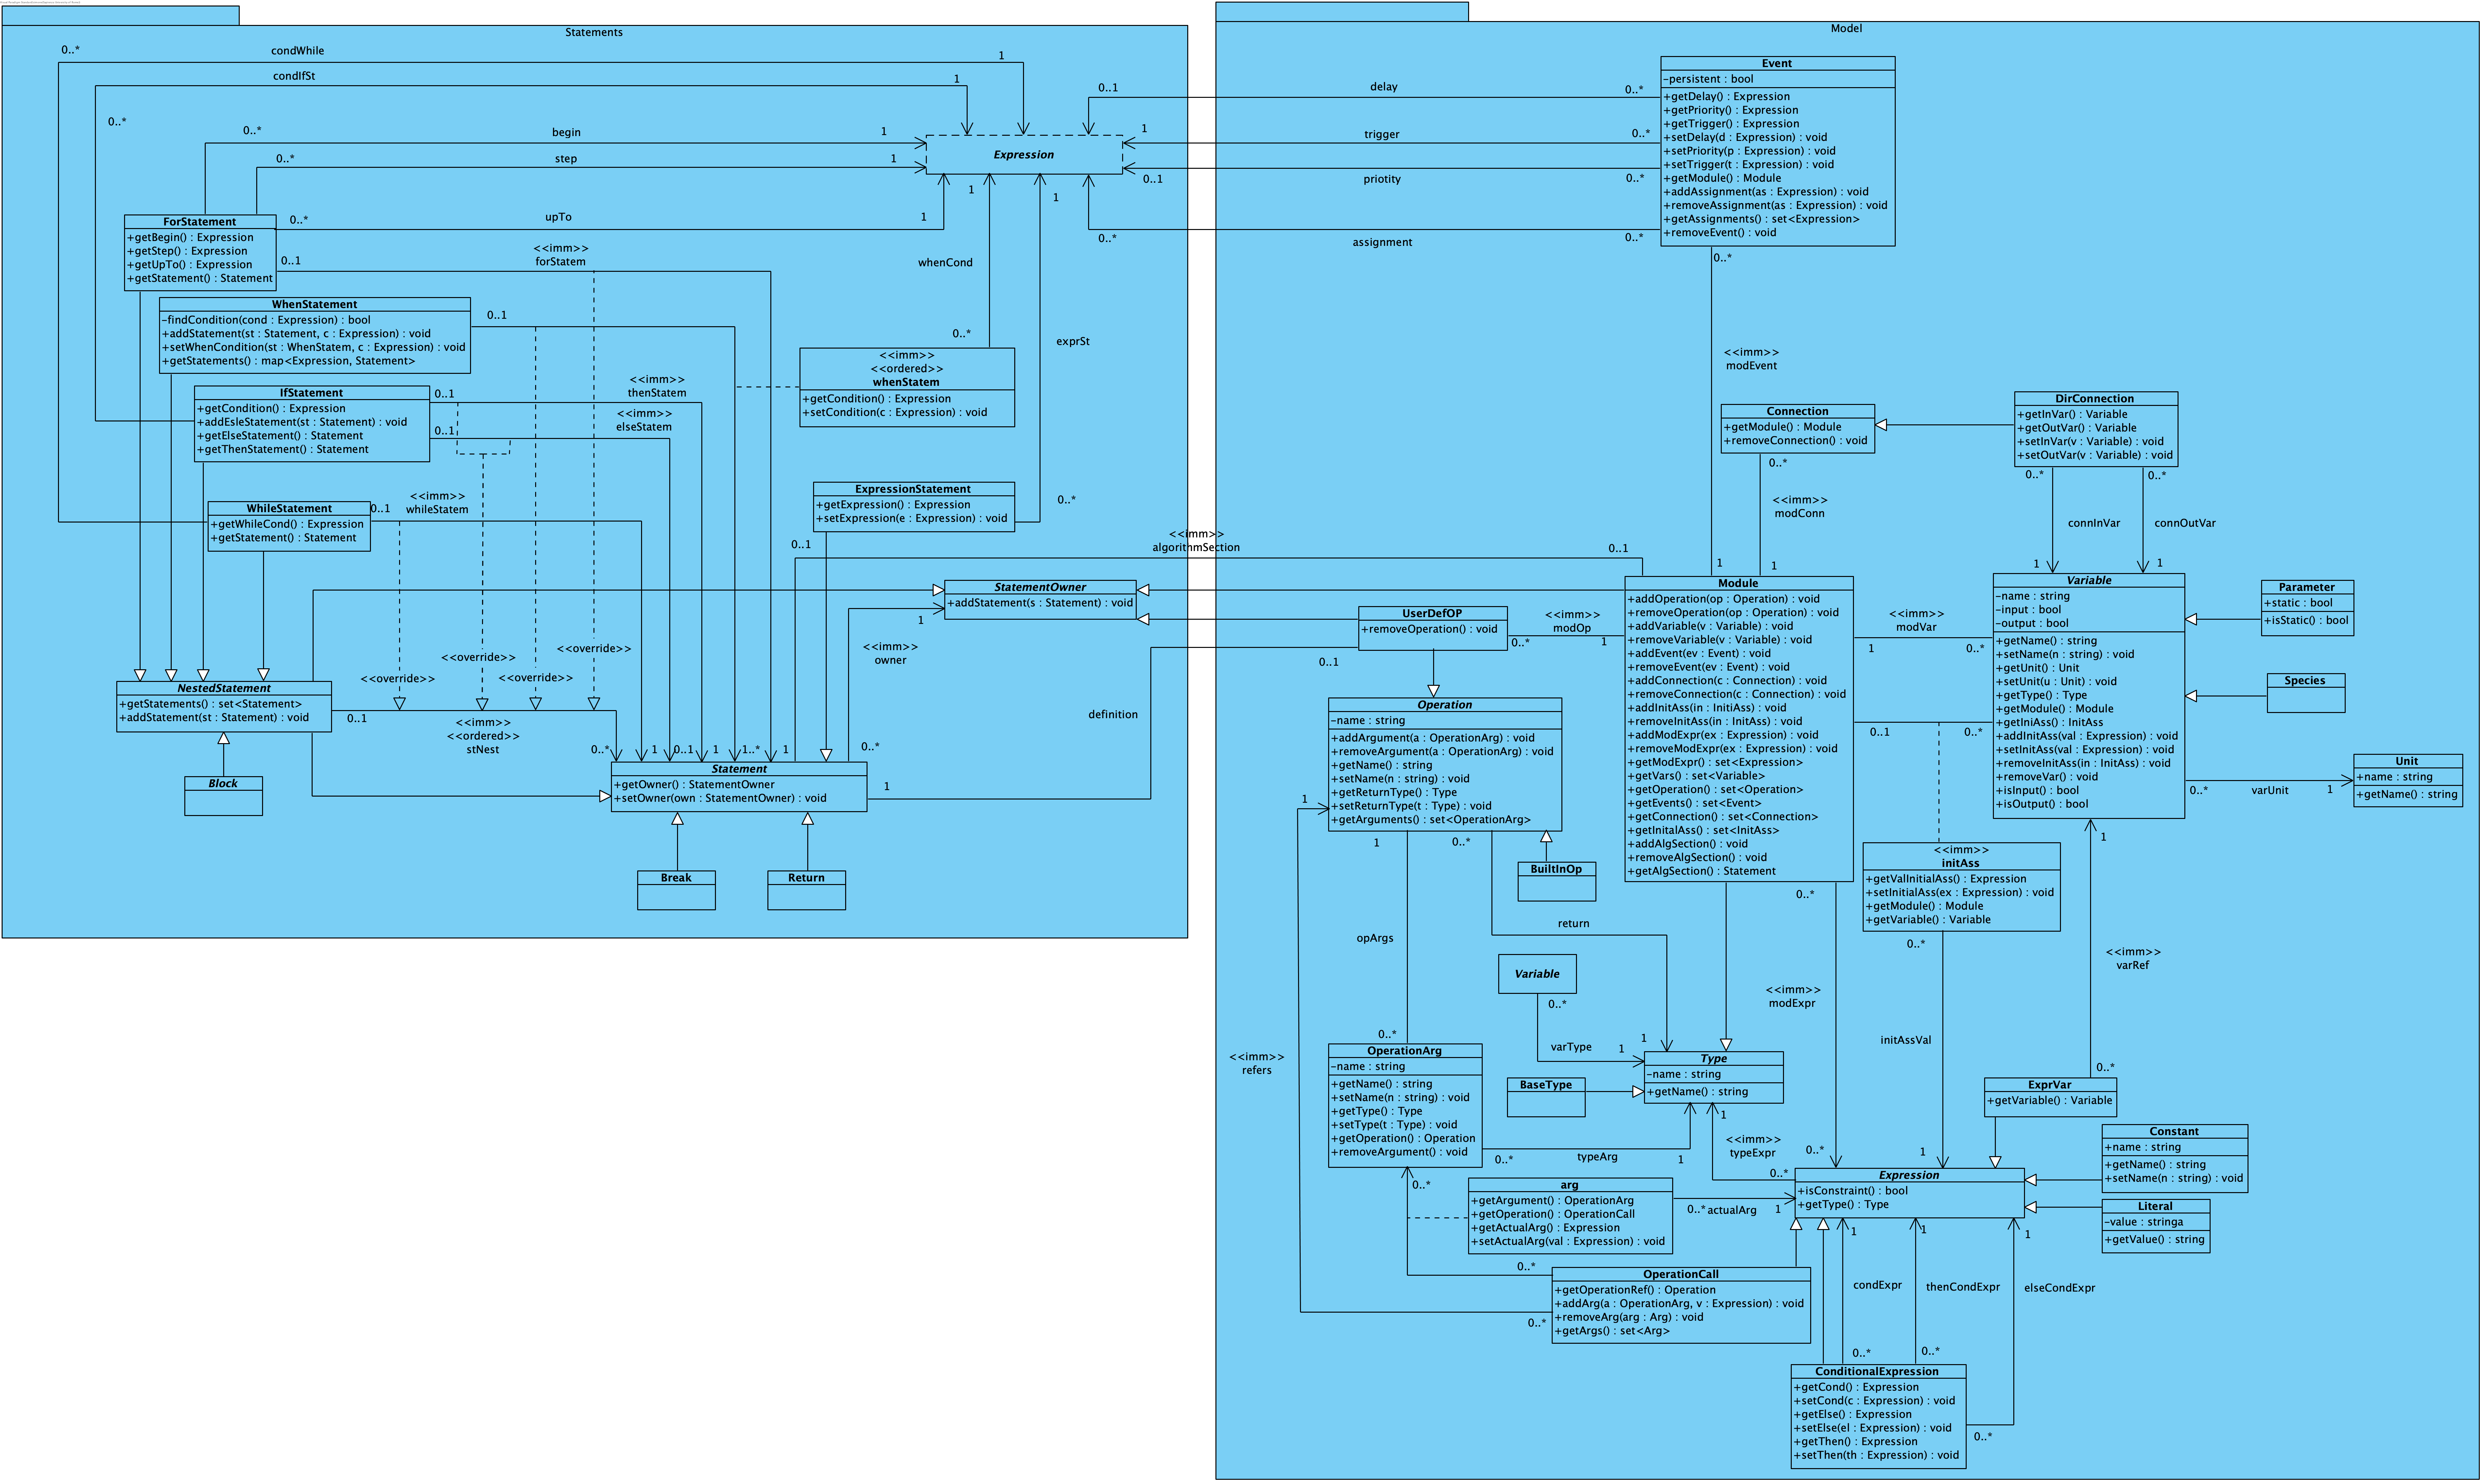
\includegraphics[width=\textwidth]{ModelsTranslatorDesign.png}
	\caption{\small{\textit{Application Design: ModelsTranslator data model.}}}
\end{figure}

\InputSection[sec:modelstranslator:design:model_design]{Package Model}{package_model/content.tex}
\InputSection[sec:modelstranslator:design:statements_design]{Package Statements}{package_statements/content.tex}
